\documentclass{standalone}
\usepackage{tikz}
\usetikzlibrary{patterns, positioning}


\begin{document}
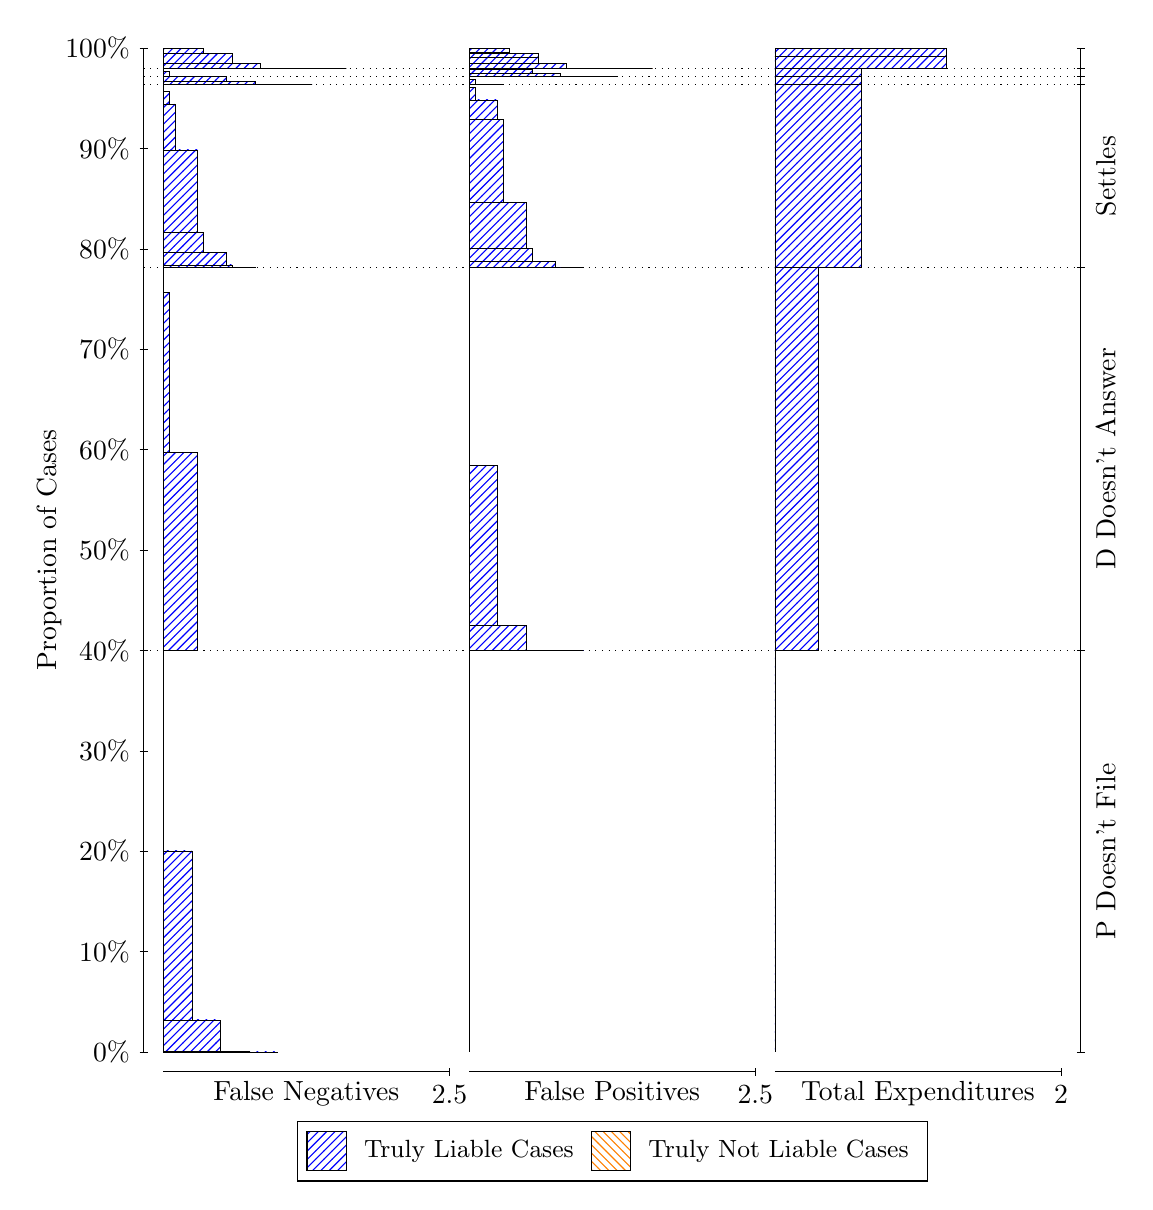
\begin{tikzpicture}
\draw[black, very thin] (1.5,1.75) -- (1.5,14.5);
\node[rotate=90, text=black, anchor=center] at (0.3, 8.125) {Proportion of Cases};
\draw[black, very thin] (1.45,1.75) -- (1.55,1.75);
\node[text=black, anchor=east] at (1.45, 1.75) {0\%};
\draw[black, very thin] (1.45,3.025) -- (1.55,3.025);
\node[text=black, anchor=east] at (1.45, 3.025) {10\%};
\draw[black, very thin] (1.45,4.3) -- (1.55,4.3);
\node[text=black, anchor=east] at (1.45, 4.3) {20\%};
\draw[black, very thin] (1.45,5.575) -- (1.55,5.575);
\node[text=black, anchor=east] at (1.45, 5.575) {30\%};
\draw[black, very thin] (1.45,6.85) -- (1.55,6.85);
\node[text=black, anchor=east] at (1.45, 6.85) {40\%};
\draw[black, very thin] (1.45,8.125) -- (1.55,8.125);
\node[text=black, anchor=east] at (1.45, 8.125) {50\%};
\draw[black, very thin] (1.45,9.4) -- (1.55,9.4);
\node[text=black, anchor=east] at (1.45, 9.4) {60\%};
\draw[black, very thin] (1.45,10.675) -- (1.55,10.675);
\node[text=black, anchor=east] at (1.45, 10.675) {70\%};
\draw[black, very thin] (1.45,11.95) -- (1.55,11.95);
\node[text=black, anchor=east] at (1.45, 11.95) {80\%};
\draw[black, very thin] (1.45,13.225) -- (1.55,13.225);
\node[text=black, anchor=east] at (1.45, 13.225) {90\%};
\draw[black, very thin] (1.45,14.5) -- (1.55,14.5);
\node[text=black, anchor=east] at (1.45, 14.5) {100\%};

\draw[black, very thin] (13.4,1.75) -- (13.4,14.5);
\draw[black, very thin] (13.35,1.75) -- (13.45,1.75);
\node[anchor=west] at (13.35, 1.75) {};
\draw[black, very thin] (13.35,6.8489) -- (13.45,6.8489);
\node[anchor=west] at (13.35, 6.8489) {};
\draw[black, very thin] (13.35,11.712) -- (13.45,11.712);
\node[anchor=west] at (13.35, 11.712) {};
\draw[black, very thin] (13.35,14.036) -- (13.45,14.036);
\node[anchor=west] at (13.35, 14.036) {};
\draw[black, very thin] (13.35,14.142) -- (13.45,14.142);
\node[anchor=west] at (13.35, 14.142) {};
\draw[black, very thin] (13.35,14.237) -- (13.45,14.237);
\node[anchor=west] at (13.35, 14.237) {};
\draw[black, very thin] (13.35,14.5) -- (13.45,14.5);
\node[anchor=west] at (13.35, 14.5) {};

\draw[black, very thin, pattern color=blue, pattern=north east lines] (1.75,1.75) rectangle (3.2033,1.75);
\draw[black, very thin, pattern color=blue, pattern=north east lines] (1.75,1.75) rectangle (2.84,1.7534);
\draw[black, very thin, pattern color=blue, pattern=north east lines] (1.75,1.7534) rectangle (2.4767,2.158);
\draw[black, very thin, pattern color=blue, pattern=north east lines] (1.75,2.158) rectangle (2.1133,4.3029);
\draw[black, very thin, pattern color=orange, pattern=north west lines] (1.75,4.3029) rectangle (1.75,4.3029);
\draw[black, very thin, pattern color=blue, pattern=north east lines] (1.75,4.3029) rectangle (1.75,6.8489);
\draw[black, very thin, pattern color=blue, pattern=north east lines] (1.75,6.8489) rectangle (2.186,9.3639);
\draw[black, very thin, pattern color=blue, pattern=north east lines] (1.75,9.3639) rectangle (1.8227,11.393);
\draw[black, very thin, pattern color=orange, pattern=north west lines] (1.75,11.393) rectangle (1.75,11.393);
\draw[black, very thin, pattern color=blue, pattern=north east lines] (1.75,11.393) rectangle (1.75,11.712);
\draw[black, very thin, pattern color=blue, pattern=north east lines] (1.75,11.712) rectangle (2.9127,11.713);
\draw[black, very thin, pattern color=blue, pattern=north east lines] (1.75,11.713) rectangle (2.622,11.745);
\draw[black, very thin, pattern color=blue, pattern=north east lines] (1.75,11.745) rectangle (2.5493,11.908);
\draw[black, very thin, pattern color=blue, pattern=north east lines] (1.75,11.908) rectangle (2.2587,12.155);
\draw[black, very thin, pattern color=blue, pattern=north east lines] (1.75,12.155) rectangle (2.186,13.206);
\draw[black, very thin, pattern color=blue, pattern=north east lines] (1.75,13.206) rectangle (1.8953,13.79);
\draw[black, very thin, pattern color=blue, pattern=north east lines] (1.75,13.79) rectangle (1.8227,13.954);
\draw[black, very thin, pattern color=orange, pattern=north west lines] (1.75,13.954) rectangle (1.75,13.954);
\draw[black, very thin, pattern color=blue, pattern=north east lines] (1.75,13.954) rectangle (1.75,14.036);
\draw[black, very thin, pattern color=blue, pattern=north east lines] (1.75,14.036) rectangle (3.6393,14.036);
\draw[black, very thin, pattern color=blue, pattern=north east lines] (1.75,14.036) rectangle (3.276,14.037);
\draw[black, very thin, pattern color=blue, pattern=north east lines] (1.75,14.037) rectangle (2.9127,14.076);
\draw[black, very thin, pattern color=blue, pattern=north east lines] (1.75,14.076) rectangle (2.5493,14.141);
\draw[black, very thin, pattern color=blue, pattern=north east lines] (1.75,14.141) rectangle (2.186,14.142);
\draw[black, very thin, pattern color=orange, pattern=north west lines] (1.75,14.142) rectangle (1.75,14.142);
\draw[black, very thin, pattern color=blue, pattern=north east lines] (1.75,14.142) rectangle (2.186,14.144);
\draw[black, very thin, pattern color=blue, pattern=north east lines] (1.75,14.144) rectangle (1.8227,14.201);
\draw[black, very thin, pattern color=orange, pattern=north west lines] (1.75,14.201) rectangle (1.75,14.201);
\draw[black, very thin, pattern color=blue, pattern=north east lines] (1.75,14.201) rectangle (1.75,14.237);
\draw[black, very thin, pattern color=blue, pattern=north east lines] (1.75,14.237) rectangle (4.0753,14.237);
\draw[black, very thin, pattern color=blue, pattern=north east lines] (1.75,14.237) rectangle (3.712,14.237);
\draw[black, very thin, pattern color=blue, pattern=north east lines] (1.75,14.237) rectangle (3.3487,14.24);
\draw[black, very thin, pattern color=blue, pattern=north east lines] (1.75,14.24) rectangle (2.9853,14.301);
\draw[black, very thin, pattern color=blue, pattern=north east lines] (1.75,14.301) rectangle (2.622,14.434);
\draw[black, very thin, pattern color=blue, pattern=north east lines] (1.75,14.434) rectangle (2.2587,14.495);
\draw[black, very thin, pattern color=blue, pattern=north east lines] (1.75,14.495) rectangle (1.8953,14.5);
\draw[black, very thin, pattern color=orange, pattern=north west lines] (1.75,14.5) rectangle (1.75,14.5);
\draw[black, very thin, pattern color=blue, pattern=north east lines] (1.75,14.5) rectangle (1.75,14.5);
\draw[black, very thin, pattern color=orange, pattern=north west lines] (5.6333,1.75) rectangle (5.6333,1.75);
\draw[black, very thin, pattern color=blue, pattern=north east lines] (5.6333,1.75) rectangle (5.6333,6.8489);
\draw[black, very thin, pattern color=orange, pattern=north west lines] (5.6333,6.8489) rectangle (7.0867,6.8489);
\draw[black, very thin, pattern color=blue, pattern=north east lines] (5.6333,6.8489) rectangle (7.0867,6.8489);
\draw[black, very thin, pattern color=blue, pattern=north east lines] (5.6333,6.8489) rectangle (6.7233,6.8494);
\draw[black, very thin, pattern color=blue, pattern=north east lines] (5.6333,6.8494) rectangle (6.36,7.1679);
\draw[black, very thin, pattern color=blue, pattern=north east lines] (5.6333,7.1679) rectangle (5.9967,9.1974);
\draw[black, very thin, pattern color=blue, pattern=north east lines] (5.6333,9.1974) rectangle (5.6333,11.712);
\draw[black, very thin, pattern color=orange, pattern=north west lines] (5.6333,11.712) rectangle (7.0867,11.712);
\draw[black, very thin, pattern color=blue, pattern=north east lines] (5.6333,11.712) rectangle (7.0867,11.713);
\draw[black, very thin, pattern color=orange, pattern=north west lines] (5.6333,11.713) rectangle (6.796,11.713);
\draw[black, very thin, pattern color=blue, pattern=north east lines] (5.6333,11.713) rectangle (6.796,11.713);
\draw[black, very thin, pattern color=blue, pattern=north east lines] (5.6333,11.713) rectangle (6.7233,11.795);
\draw[black, very thin, pattern color=blue, pattern=north east lines] (5.6333,11.795) rectangle (6.4327,11.958);
\draw[black, very thin, pattern color=blue, pattern=north east lines] (5.6333,11.958) rectangle (6.36,12.543);
\draw[black, very thin, pattern color=blue, pattern=north east lines] (5.6333,12.543) rectangle (6.0693,13.593);
\draw[black, very thin, pattern color=blue, pattern=north east lines] (5.6333,13.593) rectangle (5.9967,13.84);
\draw[black, very thin, pattern color=blue, pattern=north east lines] (5.6333,13.84) rectangle (5.706,14.004);
\draw[black, very thin, pattern color=blue, pattern=north east lines] (5.6333,14.004) rectangle (5.6333,14.036);
\draw[black, very thin, pattern color=orange, pattern=north west lines] (5.6333,14.036) rectangle (6.0693,14.036);
\draw[black, very thin, pattern color=blue, pattern=north east lines] (5.6333,14.036) rectangle (6.0693,14.038);
\draw[black, very thin, pattern color=blue, pattern=north east lines] (5.6333,14.038) rectangle (5.706,14.103);
\draw[black, very thin, pattern color=blue, pattern=north east lines] (5.6333,14.103) rectangle (5.6333,14.142);
\draw[black, very thin, pattern color=orange, pattern=north west lines] (5.6333,14.142) rectangle (7.5227,14.142);
\draw[black, very thin, pattern color=blue, pattern=north east lines] (5.6333,14.142) rectangle (7.5227,14.142);
\draw[black, very thin, pattern color=blue, pattern=north east lines] (5.6333,14.142) rectangle (7.1593,14.142);
\draw[black, very thin, pattern color=blue, pattern=north east lines] (5.6333,14.142) rectangle (6.796,14.178);
\draw[black, very thin, pattern color=blue, pattern=north east lines] (5.6333,14.178) rectangle (6.4327,14.235);
\draw[black, very thin, pattern color=blue, pattern=north east lines] (5.6333,14.235) rectangle (6.0693,14.237);
\draw[black, very thin, pattern color=orange, pattern=north west lines] (5.6333,14.237) rectangle (7.9587,14.237);
\draw[black, very thin, pattern color=blue, pattern=north east lines] (5.6333,14.237) rectangle (7.9587,14.237);
\draw[black, very thin, pattern color=orange, pattern=north west lines] (5.6333,14.237) rectangle (7.5953,14.237);
\draw[black, very thin, pattern color=blue, pattern=north east lines] (5.6333,14.237) rectangle (7.5953,14.237);
\draw[black, very thin, pattern color=orange, pattern=north west lines] (5.6333,14.237) rectangle (7.232,14.237);
\draw[black, very thin, pattern color=blue, pattern=north east lines] (5.6333,14.237) rectangle (7.232,14.241);
\draw[black, very thin, pattern color=blue, pattern=north east lines] (5.6333,14.241) rectangle (6.8687,14.302);
\draw[black, very thin, pattern color=orange, pattern=north west lines] (5.6333,14.302) rectangle (6.8687,14.302);
\draw[black, very thin, pattern color=blue, pattern=north east lines] (5.6333,14.302) rectangle (6.8687,14.303);
\draw[black, very thin, pattern color=blue, pattern=north east lines] (5.6333,14.303) rectangle (6.5053,14.386);
\draw[black, very thin, pattern color=orange, pattern=north west lines] (5.6333,14.386) rectangle (6.5053,14.386);
\draw[black, very thin, pattern color=blue, pattern=north east lines] (5.6333,14.386) rectangle (6.5053,14.435);
\draw[black, very thin, pattern color=blue, pattern=north east lines] (5.6333,14.435) rectangle (6.142,14.447);
\draw[black, very thin, pattern color=blue, pattern=north east lines] (5.6333,14.447) rectangle (6.142,14.496);
\draw[black, very thin, pattern color=blue, pattern=north east lines] (5.6333,14.496) rectangle (5.7787,14.496);
\draw[black, very thin, pattern color=blue, pattern=north east lines] (5.6333,14.496) rectangle (5.7787,14.5);
\draw[black, very thin, pattern color=blue, pattern=north east lines] (5.6333,14.5) rectangle (5.6333,14.5);
\draw[black, very thin, pattern color=orange, pattern=north west lines] (9.5167,1.75) rectangle (9.5167,1.75);
\draw[black, very thin, pattern color=blue, pattern=north east lines] (9.5167,1.75) rectangle (9.5167,6.8489);
\draw[black, very thin, pattern color=orange, pattern=north west lines] (9.5167,6.8489) rectangle (10.062,6.8489);
\draw[black, very thin, pattern color=blue, pattern=north east lines] (9.5167,6.8489) rectangle (10.062,11.712);
\draw[black, very thin, pattern color=orange, pattern=north west lines] (9.5167,11.712) rectangle (10.607,11.712);
\draw[black, very thin, pattern color=blue, pattern=north east lines] (9.5167,11.712) rectangle (10.607,14.036);
\draw[black, very thin, pattern color=orange, pattern=north west lines] (9.5167,14.036) rectangle (10.607,14.036);
\draw[black, very thin, pattern color=blue, pattern=north east lines] (9.5167,14.036) rectangle (10.607,14.142);
\draw[black, very thin, pattern color=orange, pattern=north west lines] (9.5167,14.142) rectangle (10.607,14.142);
\draw[black, very thin, pattern color=blue, pattern=north east lines] (9.5167,14.142) rectangle (10.607,14.237);
\draw[black, very thin, pattern color=orange, pattern=north west lines] (9.5167,14.237) rectangle (11.697,14.237);
\draw[black, very thin, pattern color=blue, pattern=north east lines] (9.5167,14.237) rectangle (11.697,14.397);
\draw[black, very thin, pattern color=orange, pattern=north west lines] (9.5167,14.397) rectangle (11.697,14.397);
\draw[black, very thin, pattern color=blue, pattern=north east lines] (9.5167,14.397) rectangle (11.697,14.5);
\draw[black, dotted] (1.5,6.8489) -- (13.4,6.8489);
\draw[black, dotted] (1.5,11.712) -- (13.4,11.712);
\draw[black, dotted] (1.5,14.036) -- (13.4,14.036);
\draw[black, dotted] (1.5,14.142) -- (13.4,14.142);
\draw[black, dotted] (1.5,14.237) -- (13.4,14.237);
\draw[black, very thin] (1.75,1.5) -- (5.3833,1.5);
\node[text=black, anchor=north] at (3.5667, 1.5) {False Negatives};
\draw[black, very thin] (5.3833,1.45) -- (5.3833,1.55);
\node[text=black, anchor=north] at (5.3833, 1.45) {2.5};

\draw[black, very thin] (5.6333,1.5) -- (9.2667,1.5);
\node[text=black, anchor=north] at (7.45, 1.5) {False Positives};
\draw[black, very thin] (9.2667,1.45) -- (9.2667,1.55);
\node[text=black, anchor=north] at (9.2667, 1.45) {2.5};

\draw[black, very thin] (9.5167,1.5) -- (13.15,1.5);
\node[text=black, anchor=north] at (11.333, 1.5) {Total Expenditures};
\draw[black, very thin] (13.15,1.45) -- (13.15,1.55);
\node[text=black, anchor=north] at (13.15, 1.45) {2};

\node[text=black, centered, rotate=90] at (13.72, 4.2994) {P Doesn't File};
\node[text=black, centered, rotate=90] at (13.72, 9.2806) {D Doesn't Answer};
\node[text=black, centered, rotate=90] at (13.72, 12.874) {Settles};




\draw (7.449999999999999,1.5) node[draw=none] (baseCoordinate) {};
\begin{scope}[align=center]
        \matrix[scale=0.5, draw=black, below=0.5cm of baseCoordinate, nodes={draw}, column sep=0.1cm]{
            \node[rectangle, draw, minimum width=0.5cm, minimum height=0.5cm, pattern color=blue, pattern=north east lines] {}; &
            \node[draw=none, font=\small, text=black] (B) {Truly Liable Cases}; &
            \node[rectangle, draw, minimum width=0.5cm, minimum height=0.5cm, pattern color=orange, pattern=north west lines] {}; &
            \node[draw=none, font=\small, text=black] (B) {Truly Not Liable Cases}; \\
            };
\end{scope}

\end{tikzpicture}
\end{document}